\documentclass{article}

\title{Using Linux as a development platform for Scala projects}
\date{2017-08-24}

\usepackage{amsmath}
\usepackage{graphicx}
\usepackage{verbatim}
\usepackage{cite}
\usepackage{float}
%\usepackage[backend=bibtex, style=verbose-trad2]{biblatex}
%\bibliography{MyLibrary}

\author{Roxana Tesileanu \\ 
\\ 
roxana.te@web.de \\
INCDS, Romania }

\begin{document}
	\pagenumbering{gobble} 
	\maketitle
	\newpage
	\pagenumbering{arabic}

\tableofcontents
\newpage

\section{Introduction}

This is your instructor \footnote{\label{footnote1}Picture \ref{fig: Roxi} was taken before my sommer break.} : 
\\
\begin{figure} [H]
 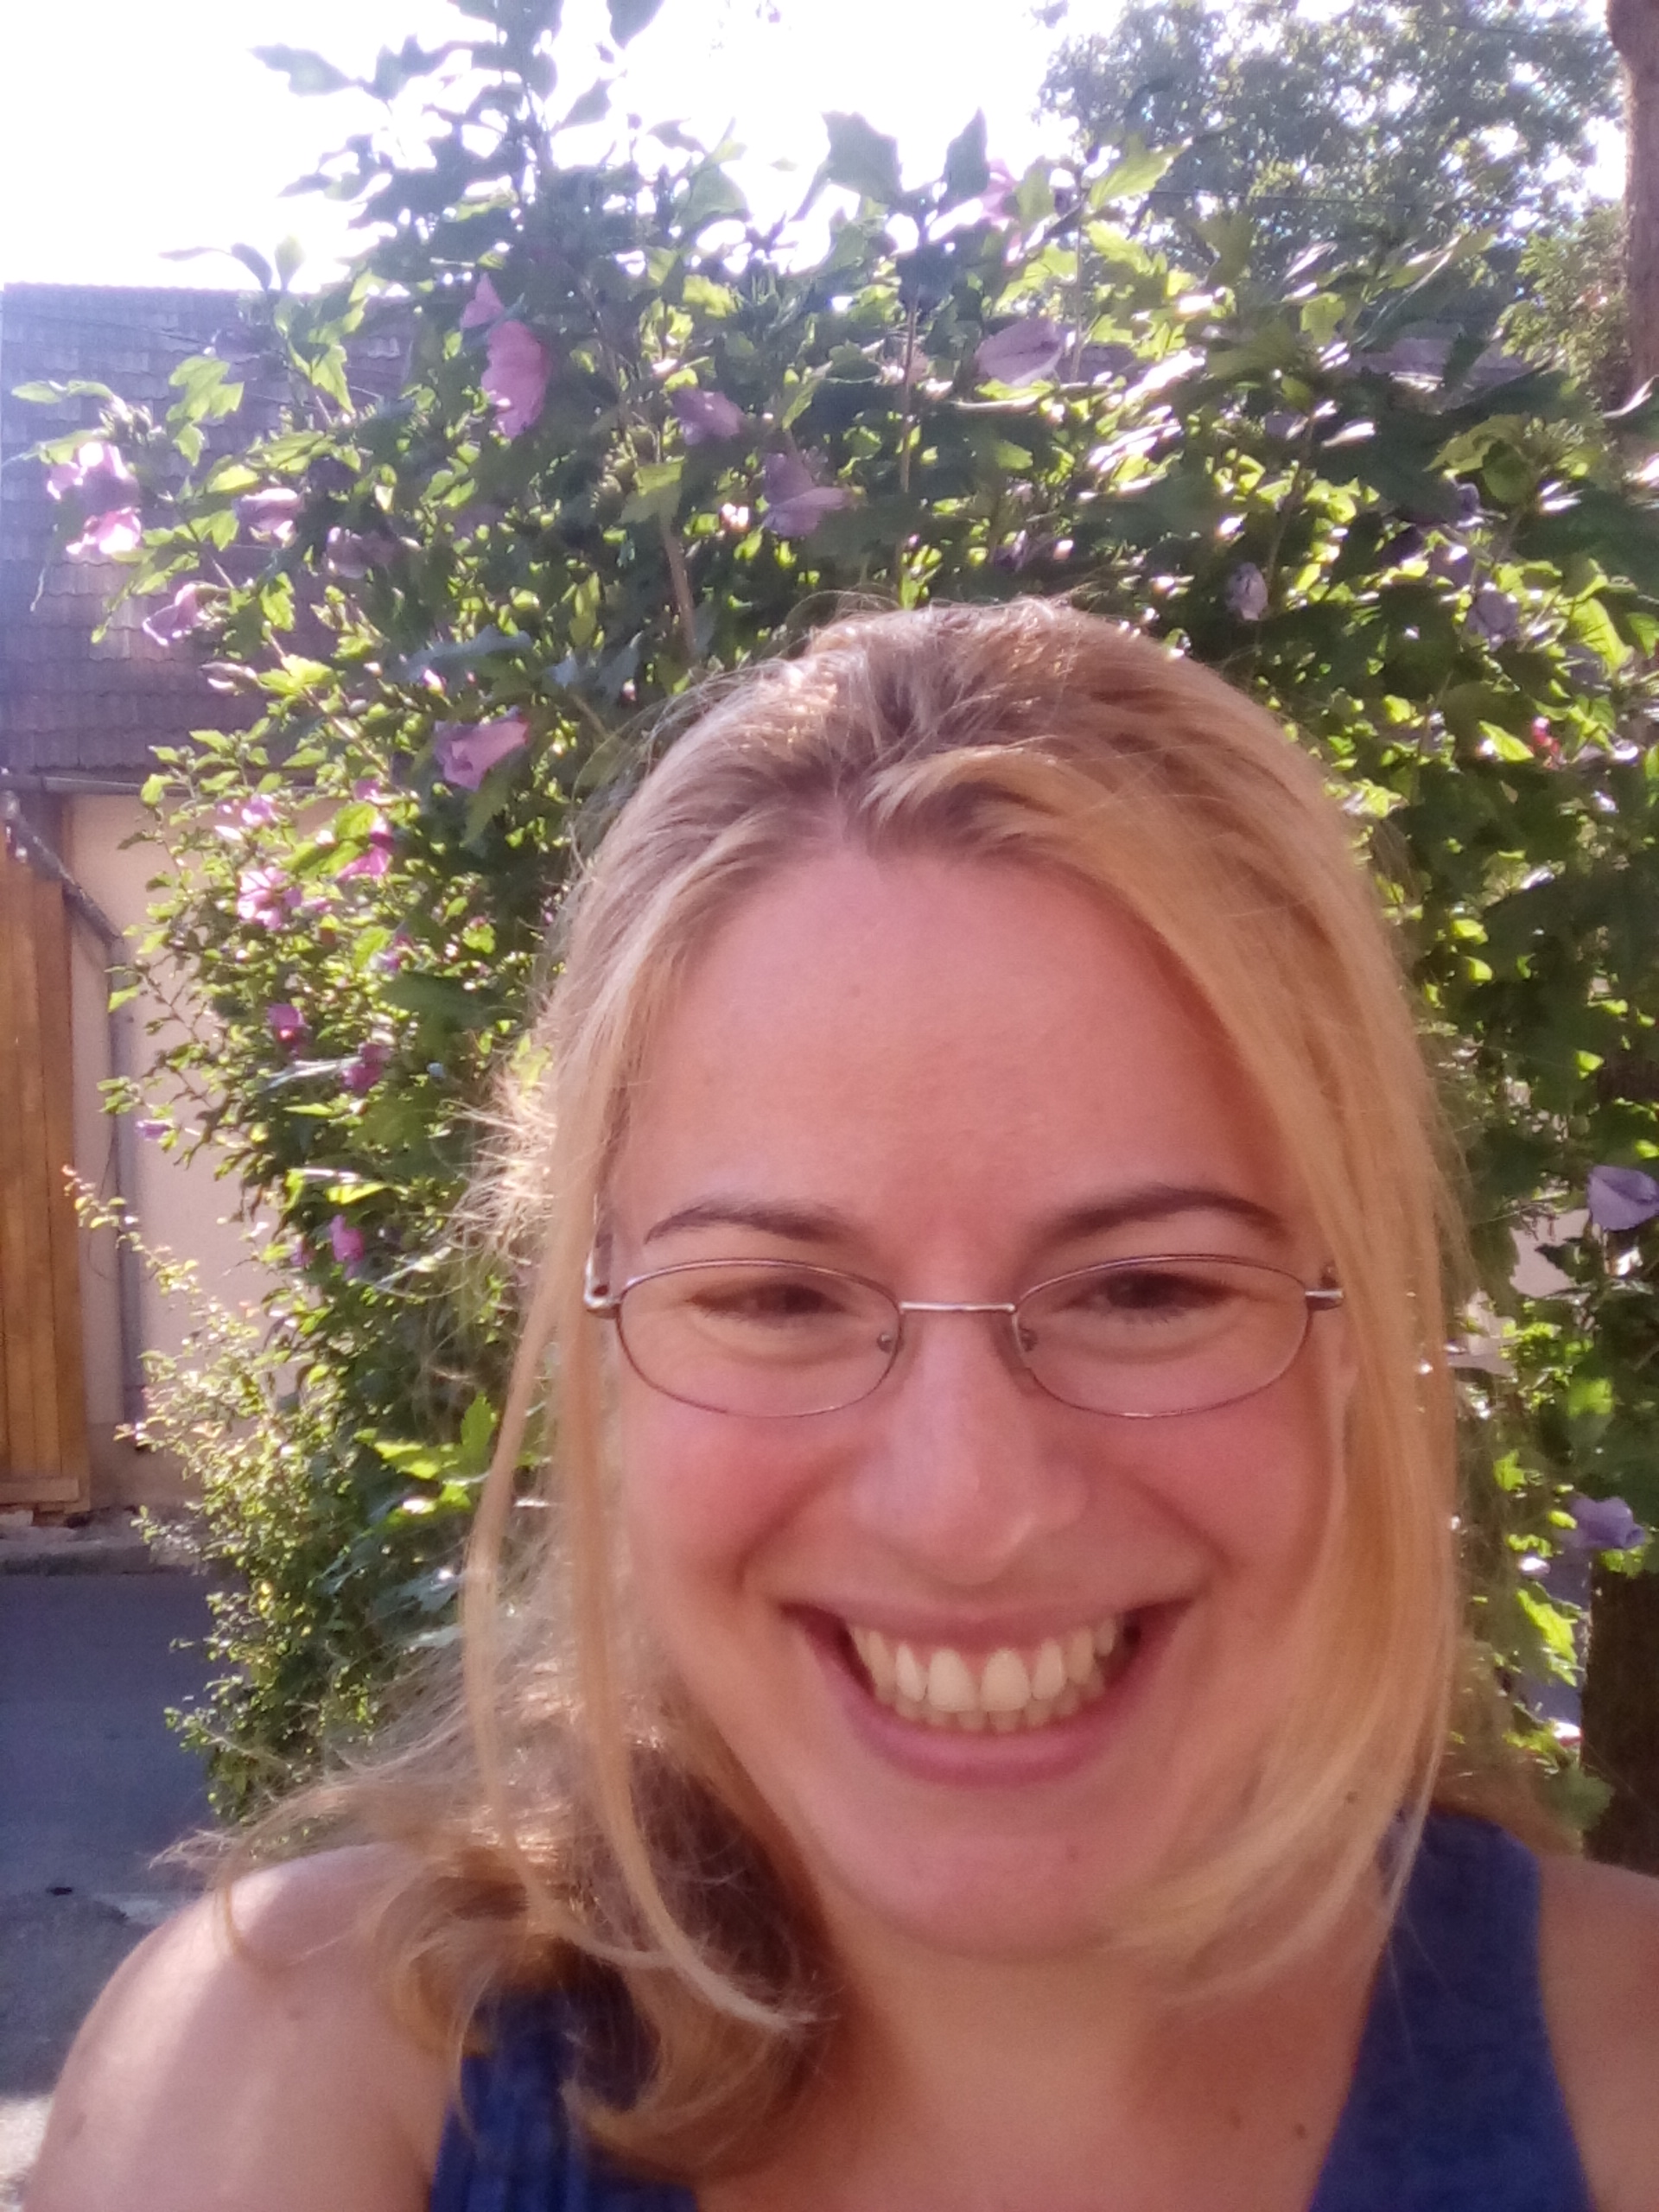
\includegraphics[width=\linewidth]{eu_institut.jpg}
 \caption{Me}
 \label{fig: Roxi}
\end{figure}


\newpage
A random citation looks like this:
\cite{odersky_programming_2010}. This is embedded in text. \\
%\autocite[1]{odersky_programming_2010}
The components of a development system are (Rehman and Paul, 2003, p.10):\newline
- hardware platform \\
- operating system \\
- editors \\
- compilers and assemblers \\
- debuggers \\
- version control system \\
- bug tracking \\

.....

This formula $f(x) = x^2$ is an example.
\begin{equation}
\left[
\begin{matrix}
1 & 0 \\
0 & 1
\end{matrix}
\right]
\end{equation}

\begin{equation}
\int^a_b\frac{1}{3}x^3
\end{equation}

\begin{equation}
\theta = \int^1_0 f(x)
\end{equation}
\\

\begin{table}[h!]
\centering
\caption{ANOVA Sums-of-squares.}
\label{tab: table1}
\begin{tabular}{l|c|r}

Residual SS & Groups SS & Total SS \\
\hline
1 & 3 & 4 \\

\end{tabular}
\end{table}





\section{Using vim as an editor for the Scala code}
\section{Using SBT}
\subsection{Installing SBT}
\subsection{Creating a Scala project}
\subsection{Some SBT functionalities}
\section{References}

\bibliography{MyLibrary}
\bibliographystyle{plain}
%\printbibliography
\section{Appendix}
\begin{appendix}

Additional information comes here.
\listoffigures
\listoftables

\end{appendix}

  
\end{document}


